%!TEX TS-program = xelatex
%!TEX encoding = UTF-8 Unicode

%%%  Syllabus template for use with style files at http://kjhealy.github.com/latex-custom-kjh
%%%  Kieran Healy

\documentclass[11pt,article,oneside]{memoir}

% packages
\usepackage{org-preamble-xelatex}
\usepackage{wallpaper}
\usepackage{xcolor}
\usepackage{enumitem}
\usepackage{multicol}
\setlength{\columnsep}{1em}
\usepackage{booktabs}
\newcommand{\ra}[1]{\renewcommand{\arraystretch}{#1}}

\AtBeginBibliography{\small}

% Definitions
\def\myauthor{Author}
\def\mytitle{Title}
\def\mycopyright{\myauthor}
\def\mykeywords{}
\def\mybibliostyle{plain}
\def\mybibliocommand{}
\def\mysubtitle{}
\def\myaffiliation{Louisiana State University}
\def\myaddress{309 Design}
\def\myemail{baharmon@lsu.edu} 
\def\myweb{https://baharmon.github.io/}
\def\myphone{919.622.8414}
\def\myversion{}
\def\myrevision{}
\def\myaffiliation{\ \\Louisiana State University}
\def\myauthor{Brendan Harmon}
\def\mykeywords{Landscape Architecture, Syllabus}
\def\mytitle{{\normalsize \textsc{LA} 7061 \newline \newline} \Large \bfseries Advanced Topics Studio \newline} 
\def\mysubtitle{\large Serious gaming \newline \newline \tiny for \bfseries JEAN LAFITTE}

% color
\makeatletter
\newcommand{\globalcolor}[1]{%
  \color{#1}\global\let\default@color\current@color
}
\makeatother

% begin
\begin{document}

\setlength\bibitemsep{0.75em}

% fonts
\defaultfontfeatures{}
\defaultfontfeatures{Scale=MatchLowercase}         
\setmainfont[Scale=1, Path = fonts/lato/,BoldItalicFont=Lato-RegIta,BoldFont=Lato-Reg,ItalicFont=Lato-LigIta]{Lato-Lig}
\setsansfont[Scale=1, Path = fonts/lato/,BoldItalicFont=Lato-RegIta,BoldFont=Lato-Reg,ItalicFont=Lato-LigIta]{Lato-Lig}
\setmonofont[Mapping=tex-text,Scale=0.8,Path = fonts/inconsolata/]{i}

\def\ind{\hangindent=1 true cm\hangafter=1 \noindent}
\def\labelitemi{$\cdot$}
\chapterstyle{article-4-sans}  
\title{\LARGE \mytitle \newline \mysubtitle}     
\author{\large\myauthor \newline \footnotesize\texttt{\noindent\myemail}}
\date{\normalsize Spring 2018. Design 309.\newline Monday, Wednesday, \& Friday \newline 9:30am--11:30am.}
\published{\,}

% -------------------------------- COVER PAGE -------------------------------- 

\pagenumbering{gobble}
\globalcolor{black}
\vspace*{-10em}
\maketitle
\setlength{\wpXoffset}{-4em}
\ThisCenterWallPaper{1.6}{../images/specimen_planting_3_cutout.jpg}
\vfill
%\begin{center}
%\noindent \textbf{...} \\
%\copyright \hspace*{0.25em} ... \\
%\end{center}
\clearpage

% -------------------------------- DESCRIPTION -------------------------------- 

\pagenumbering{arabic}
\globalcolor{black}
\vspace*{-10em}
\maketitle

\section{Course description}
%
In this studio you will design and develop serious games
that explore the challenges of coastal change
for the town of Jean Lafitte in Jefferson Parish, Louisiana.   
%
These games will use Tangible Landscape
-- a tangible interface for GIS -- 
to model, simulate, and visualize alternative future scenarios. 
%
The games will address the impact of coastal change 
-- of storm surge, flooding, erosion, and land-loss --
on Jean Lafitte. 
%
The games will explore how methods for defense or adaptation 
such as levee construction, elevated buildings, floating buildings, 
and bioretention wetlands 
perform in simulated storms. 
%
You will  run a serious gaming workshop
for the community in Jean Lafitte
and another for the LSU College of Art and Design. 

%\clearpage

% -------------------------------- SCHEDULE -------------------------------- 

\section{Course schedule}
\normalsize

\begin{multicols}{3}
\begin{enumerate}[label=\textbf{\arabic*}]
\small
%
\item Introduction
\item Terrain modeling
\item Digital fabrication
\item Mapping
\item Storyboarding I
\item Storyboarding II
\item Python I
\item Python II
\item Game design I
\item Game design II
\item Game design III
\item Booklet
\item Rehearsal
\item Workshop I
\item Workshop II
%
\end{enumerate}
\end{multicols}

\clearpage

% -------------------------------- PROJECTS -------------------------------- 
\section{Projects}
As groups of 5 you will
design and develop a serious game using Tangible Landscape
that explores coastal change in the town of Jean Lafitte.
\\

\noindent \textbf{Models}
Each group will make a hollow CNC-milled
terrain model of the town  in high density foam.
These models will be used to cast sand models. 
Each group will also 3D print the town's buildings. 
\\

\noindent \textbf{Game}
Each group will design and develop a game
using Tangible Landscape. 
Their game will explore a set of scenarios
for coastal change, defense, and adaptation. 
\\

\noindent \textbf{Posters}
Each group will design and print posters
for the serious gaming workshops. 
The posters should 
include maps and imagery of Jean Lafitte,
maps and visualizations of 
coastal change scenarios for the town,
and introduce their game.
\\

\noindent \textbf{Booklet}
Each group will prepare a booklet for the serious gaming workshops
that describes the challenges of coastal change 
and explains the rules of the game.
The booklets should include a survey 
for participants to complete.
\\

\noindent \textbf{Workshops}
All of the groups will present their games at 
a community workshop in Jean Lafitte
and another workshop at the LSU College of Design. 
In the workshop participants will play the games
and develop their own design solutions.
\\

% -------------------------------- Grading -------------------------------- 
\section{Grading}

\begin{table}[H]
\small
\begin{tabular}{l l l l l l l l l l}
\textbf{Models} & 20\% &
\textbf{Game} & 20\% &
\textbf{Posters} & 20\% &
\textbf{Booklet} & 20\% &
\textbf{Workshops} & 20\% \\
\end{tabular}
\end{table}

% -------------------------------- Readings -------------------------------- 
\section{Readings}
\renewcommand*{\bibfont}{\normalsize} %\small
\vspace*{0.5cm}
\nocite{*}
\setlength\bibitemsep{1\baselineskip}
\printbibliography[heading=none]

\clearpage

% -------------------------------- Software -------------------------------- 
\section{Software}
GRASS GIS | \url{https://grass.osgeo.org/}\\
Blender | \url{https://www.blender.org/}\\
Rhinoceros | \url{https://www.rhino3d.com/}\\
RhinoTerrain | \url{http://www.rhinoterrain.com/}\\
RhinoCAM | \url{https://mecsoft.com/rhinocam-software/}\\
ArcGIS | \url{http://desktop.arcgis.com/en/}\\


% -------------------------------- Figures -------------------------------- 

\begin{figure}[H]
\begin{center}
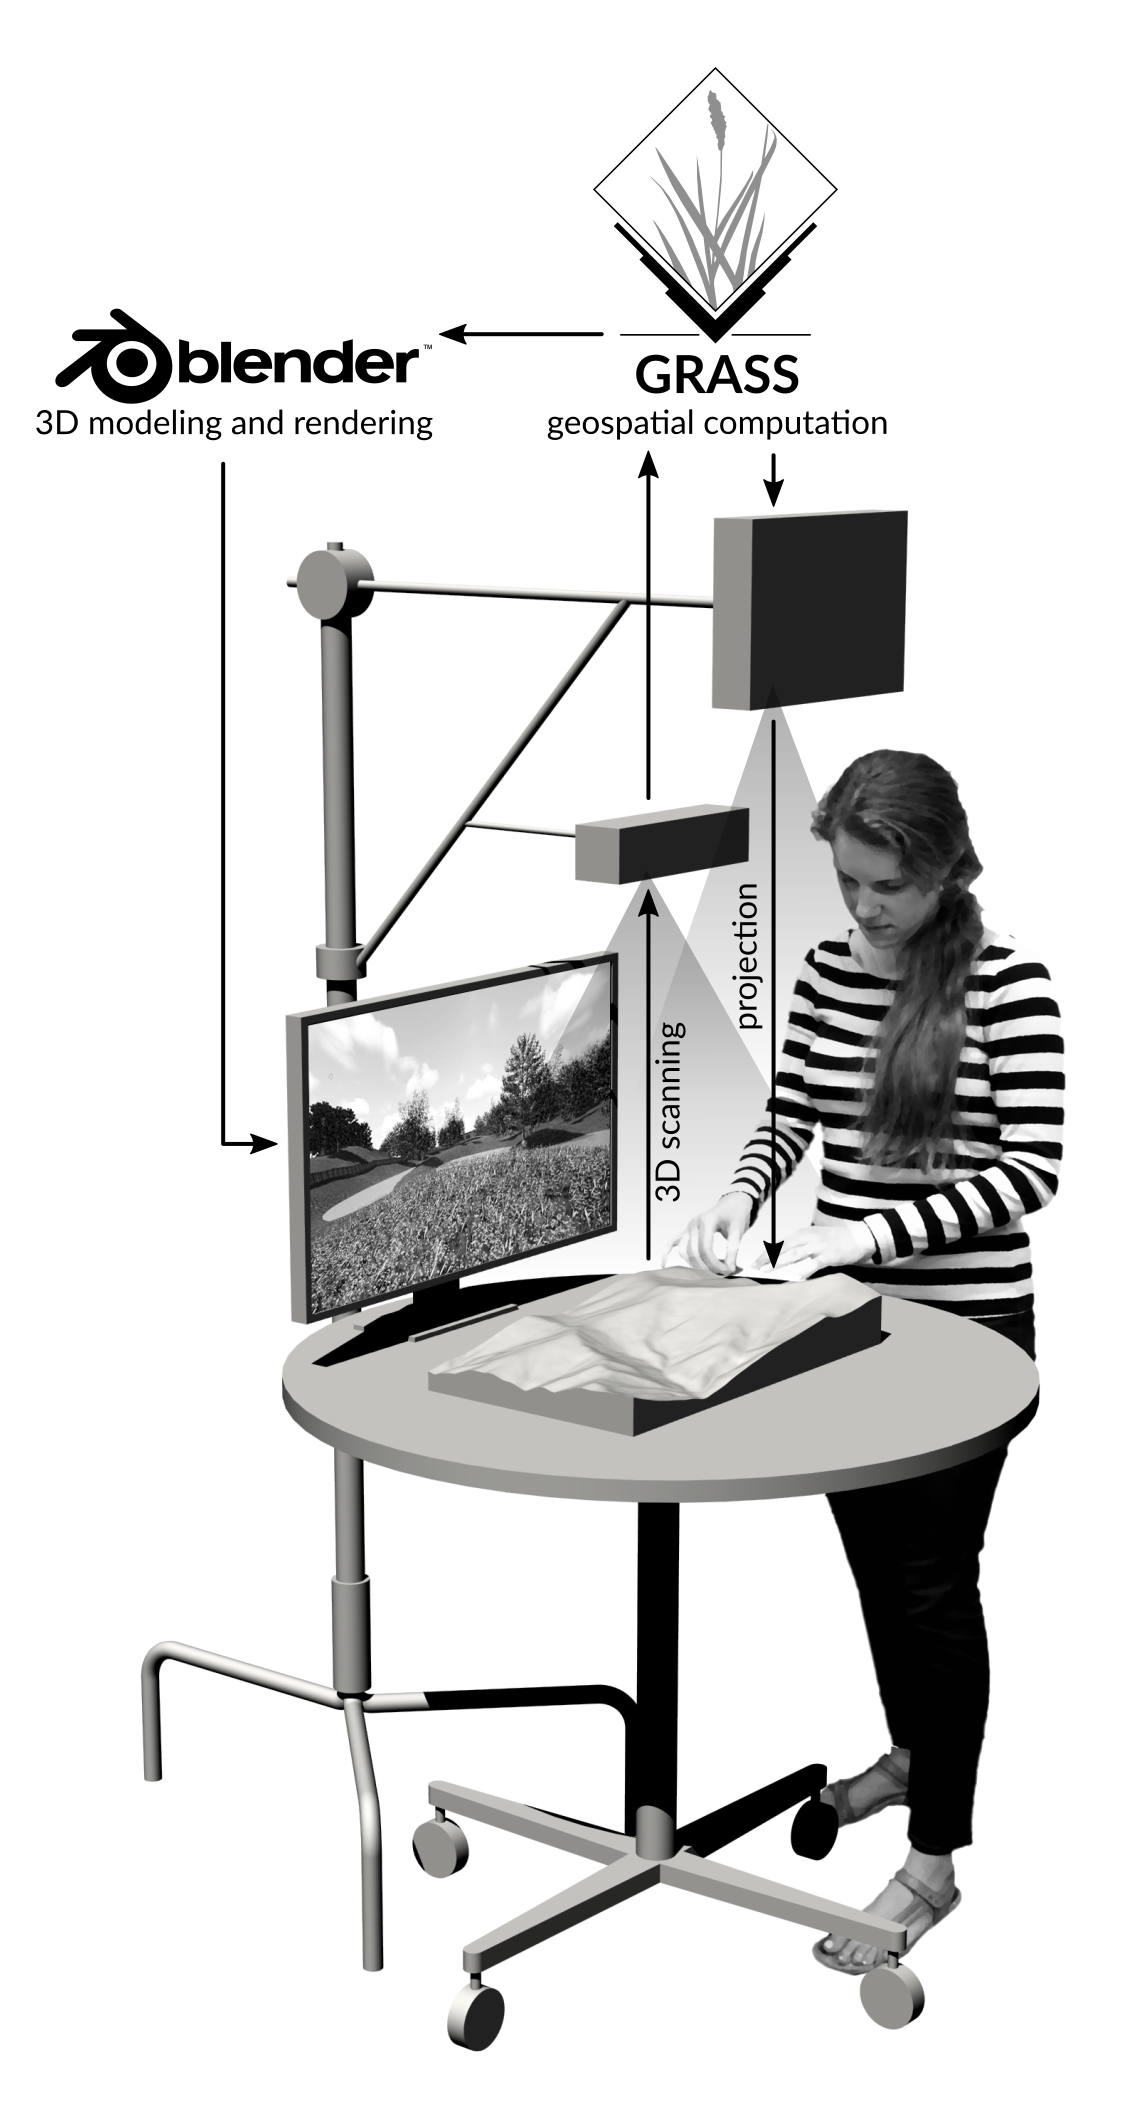
\includegraphics[width=0.5\textwidth]{../images/rendered_diagram_2.png}
\caption{Tangible Landscape | \url{http://tangible-landscape.github.io/}}
\label{fig:tangible_landscape}
\end{center}
\end{figure}

\clearpage

% -------------------------------- Policies -------------------------------- 
\section{Policies}

\noindent \textbf{Time Commitment Expectations}
LSU's general policy states that for each credit hour, you (the student) should plan to
spend at least two hours working on course related activities outside of class. Since this course is for six credit hours, you should expect to spend a minimum of twelve hours outside of class each week working on assignments for this course. For more information see: 
\url{http://catalog.lsu.edu/content.php?catoid=12&navoid=822}.\\

\noindent \textbf{LSU student code of conduct}
The LSU student code of conduct explains student rights, excused absences, and what is expected of student behavior. Students are expected to understand this code:  \url{http://students.lsu.edu/saa/students/code}.\\ %Any violations of the LSU student code will be duly reported to the Dean of Students.\\

\noindent \textbf{Disability Code}
The University is committed to making reasonable efforts to assist individuals with disabilities in
their efforts to avail themselves of services and programs offered by the University. To this end,
Louisiana State University will provide reasonable accommodations for persons with
documented qualifying disabilities. If you have a disability and feel you need accommodations in
this course, you must present a letter to me from Disability Services in 115 Johnston Hall,
indicating the existence of a disability and the suggested accommodations.\\

\noindent \textbf{Academic Integrity}
According to section 10.1 of the LSU Code of Student Conduct, ``A student may be charged with Academic Misconduct'' for a variety of offenses, including the following: unauthorized copying, collusion, or collaboration; ``falsifying'' data or citations; ``assisting someone in the commission or attempted commission of an offense''; and plagiarism, which is defined in section 10.1.H as a ``lack of appropriate citation, or the unacknowledged inclusion of someone else's words, structure, ideas, or data; failure to identify a source, or the submission of essentially the same work for two assignments without permission of the instructor(s).''\\

\noindent \textbf{Plagiarism and Citation Method}
Plagiarism is the ``lack of appropriate citation, or the unacknowledged inclusion of someone else's words, structure, ideas, or data; failure to identify a source, or the submission of essentially the same work for two assignments without permission of the instructor(s)'' (Sec. 10.1.H of the LSU Code of Student Conduct). As a student at LSU, it is your responsibility to refrain from plagiarizing the academic property of another and to utilize appropriate citation method for all coursework. In this class, it is recommended that you use Chicago Style author-date citations. Ignorance of the citation method is not an excuse for academic misconduct.

\end{document}
